The lecture beings by a rather basic observation that around 90\% of US elections at most levels of government are won by the incumbent party.

\begin{SCfigure}[][h]
    \raggedleft
    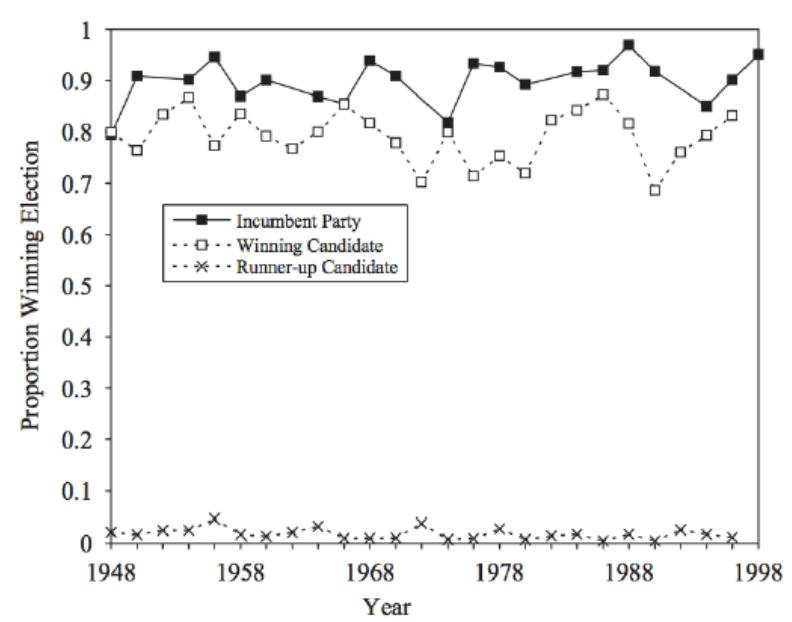
\includegraphics[width=0.6\textwidth]{figures/lee2008.png}
    \caption{\textbf{Incumbency advantage} The figure shows the share of election won by candidates of incumbent and runner up parties. From \cite{lee_randomized_2008}}
    \label{fig: incumbency}
\end{SCfigure}

The challenge with answering if incumbency causally affects the probability of winning is that there is no good random variation to use. After all randomly changing around which politicians are incumbent would be infeasible. Instead one can use a regression discontinuity design to extract the causal component. In particular we might worry that some districts simply lean either Republican or Democrat and this is what causes the large gap in election probabilities for incumbents, not the incumbency itself.

\citeauthor{lee_randomized_2008} does exactly this. They set up a RD design using data from elections for the US house of representatives from 1946 to 1998. In each distict they then calculate the democratic vote margin $V$ in election at time $t$ as a running variable (if this is above 0 democrats win, if it is below republicans win). Using this they create a "treatment" of $D=(V>0.5)$ i.e. treatment is a democrat being incumbent in the period $t+1$ election. As outcome they have outcomes of the period $t+1$ election.

They also gather a long list of covariates $X$ which are determined prior to the period $t$ election (i.e. from year $t-1$ or earlier).

The authors find that the true causal effect of incumbency is somewhere between a 5 and 10\% increase in the vote share and a corresponding 36\% increase in probability of winning the election. Notice however that this setup defines winning at a party level, so while having a democratic incumbent increases the probability of a democrat being elected, it is uncertain if this effect also exists at the individual level. 

To study if individual incumbency or party incumbency is the driving force is a different and harder question to answer, since there is no simple cutoff determining if a politician decides to run again, or attempts to pass the position on to another party member.

\subsection{Regression discontinuity}
RD designs are based on the existence of some running variable $V$ with an observed threshold $v_0$ above which the treatment (i.e. winning the previous election) is given. The basic idea is then that around the threshold $[v_0 - \epsilon, v_0 + \epsilon]$ it is essentially random which party ends up on either side, and we can get an estimate of the causal effect of incumbency. This can be done either by running the regression only on observations where $V\in[v_0 - \epsilon, v_0 + \epsilon]$ or by adding a function $g(V)$ to the regression which is flexible enough to capture any nonlinearities outside the interval. Note that the RD design doesn't estimate the full ATE, but only ATE* which is a weighted ATE with high weight on observations close to $v_0$. 

One might suspect that even close to $v_0$ parties have influence on who wins, but as long as there is some element of randomness in who actually wins the procedure will work. Given the RD estimates the correct result we can also infer that any predetermined characteristics of the running parties should be continuous around $v_0$, in other words there should not be any discontinuities in other variables $X$ which were determined before the election. Checking if this is the case is esentially a test of random assignment around the threshold.